%************************************************
\chapter{Design}\label{ch:design}
%************************************************
In this section we will present in details the possibilities and choices involved in accommodating the goals of this system. We start out by defining the requirements of the framework. We discuss briefly the the challenges of building onto some of the related systems. Next, we define the overall architecture of the system that can accommodate the requirements. We detail the possibilities and choices for major component of the Simulation Designer and the Simulation Runtime. We conclude this chapter with the final design of the framework.

%************************************************
\section{Requirements} % (fold)
\label{sec:requirements}
%************************************************
In Section \ref{sec:goal} we have defined the main goals of the system as a list of high level system requirements. They are very generic and hard to establish an architecture upon. Because they do not contain details of the functionality the end-user of the system will be able to use. To have a clear vision of what this system needs to achieve, we will defined in this section a list of requirements from the end-user's perspective.\\

We have decided to use the user stories concept\cite{cohn2004user}, as a way to express the requirements of this system.\\

Agile Software Development is an iterative and incremental software development methodology, promoting adaptive planning, evolutionary development and delivery, while encouraging rapid and flexible response to change \cite{agile:online}. It is mainly used in the industry. One of the best practices in Agile Software Development for requirements is \emph{user stories}. We have not employed Agile Software Development in this work, but we have used the user stories concept as the agile methodology and the iterative design process resemble similarities and applying the user stories in this context, comes naturally.\\

''A user story describes functionality that will be valuable to either a user or purchaser of a system or software'' \cite{cohn2004user}. User stories are written from the perspective of the system's users. A specific group of users, will use the system in a certain way; the feature requested by this group represents a \emph{user role}. The user role does not necessarily have to be assigned to a human user; it can also be an external service in need of accessing some data.\\

%************************************************
\subsection{User Roles}\label{subsec:user_roles}
%************************************************
Writing the requirements following the user story concept, helps us reflect upon the needs this framework must satisfy, from the user's perspective. Based on the goals of the system defined in Section \ref{sec:goal} and supported by the use case scenario defined in Section \ref{sec:scenario}, we have first identified the user roles for this framework:
\begin{table}[H]
	\begin{center}
		\small \begin{tabular*}{1.1\columnwidth}{p{3cm}p{3cm}p{5.5cm}} 
			\\ \hline \hline
			Role & Who & Role Description \\ \hline \hline

		 	System Designer & The researcher & As discussed in the introduction \ref{ch:introduction}, someone designing a mobile context-aware system based on the egocentric interaction paradigm. Uses the framework to design a simulation of the egocentric system.\\ \hline

		 	Simulation User & The researcher, a QA engineer, an end-user of the egocentric system & This role can be fulfilled by users interested in the resulting egocentric system.\\ \hline

		 	Third Party Service & An individual piece of software & An individual piece of software that builds business logic based on the monitored context data, as the simulation unfolds.\\ \hline
		\end{tabular*}
		
		\caption{List of roles for the EgoSim framework}
		\label{table:roles}
	\end{center}
\end{table}
The ''who'' presents the possible user types that can fulfil a specific role, while the ''description'' briefly describes the role's main interest in the system.\\
% section user_roles (end)

%************************************************
\subsection{User Stories}\label{subsec:user_stories}
%************************************************
The following list of user stories, represent the requirements of the EgoSim framework:
\begin{enumerate}
	\item[\textlabel{1.}{us:1}] \emph{As a system designer, I want to model the environment my egocentric system will run in. The environment's model has to be populated with everyday physical objects and devices}. It is part of goal \ref{goal:1} and presented as a need in points \ref{scenario:1}, \ref{scenario:1A}, \ref{scenario:1B} and \ref{scenario:1C}.

	\item[\textlabel{2.}{us:2}] \emph{As a system designer, I need to identify the objects I want to be monitored during the simulation}, as described in goal \ref{goal:2} and point \ref{scenario:1D} in the scenario.

	\item[\textlabel{2.1}{us:2.1}] \emph{As a system designer, I want to specify how certain entities can be interacted with}. Points \ref{scenario:1E}, \ref{scenario:1F}, \ref{scenario:1G} and \ref{scenario:1H} illustrate a few ways entities could be interacted with.

	\item[\textlabel{2.2.}{us:2.2}] \emph{As a system designer, I want to augment objects that will be monitored with information needed by the SSM model}, as illustrated in point \ref{scenario:1I}. In order for the SSM classification to work, it needs to be aware of specific parameters for each entity. By default, each monitored entity will carry a set of default SSM configuration data, but certain entities might need some adjusted values. The SSM configuration parameters are detailed in Section \ref{subsec:ssm_params}.

	\item[\textlabel{3.}{us:3}] \emph{As a system designer, I want to run a simulation based on the environment model I have set up}.

	\item[\textlabel{4.}{us:4}] \emph{As a simulation user, I want to control a virtual avatar within the simulated environment}. This behaviour is mentioned in goal \ref{goal:1} and, as described in points \ref{scenario:2}, \ref{scenario:2A}, \ref{scenario:2B} and \ref{scenario:2C}, I want to be able to control the movement and field of vision of the agent. Also, I want to be able to pick up certain objects, carry them around and make them interact with other objects (e.g. put it down on a surface).

	\item[\textlabel{5.}{us:5}] \emph{As a simulation user, I want to have a sense of reality in the simulated environment}. The user should comprehend and fell present in the target environment.

	\item[\textlabel{6.}{us:6}] \emph{As a system designer, I want the simulation to classify monitored objects into SSM sets as the agent is being controlled}. This requirement is mentioned in goal \ref{goal:2} and highlighted in the scenario throughout points \ref{scenario:2D} and \ref{scenario:2E}. The SSM sets are detailed in Section \ref{subsec:ssm_params}.

	\item[\textlabel{7.}{us:7}] \emph{As a third party service, I want to access the content of SSM sets through a publicly available API from within the simulation}. Goal \ref{goal:3} covers this requirement, while point \ref{scenario:3} describes a useful scenario.

	\item[\textlabel{8.}{us:8}] \emph{As a simulation user, I want to follow the state of SSM sets, in real time, as the simulation unfolds}. As described in goal \ref{goal:3}, this requirement satisfies the need for an ''easy way to visualize the SSM spaces in real-time''.

\end{enumerate}

While an extra requirement is needed to fully support the situative space model - namely, representation of and interaction with virtual objects - we leave that requirement for future work.\\
% section user_stories (end)

%************************************************
\subsection{Non-functional Requirements}\label{subsec:nfrs}
%************************************************
To strengthen the requirements above, we conclude this section with a list of non-functional requirements (NFRs)\footnote{constraints on the system's behaviour}:
\begin{table}[H]
	\begin{center}
		\small \begin{tabular*}{1.1\columnwidth}{p{10cm}p{1.5cm}} 
			\\ \hline \hline
			NFR & Relates to \\ \hline \hline

		 	The agent should not be able to pass through walls and other objects in the environment. & \ref{us:4}\\ \hline

		 	The visualization of simulated environment should be non-blocking. No matter how heavy are the computations carried out under the hood, the simulation user's experience should not be affected. & \ref{us:5}\\ \hline

		 	Only objects within the field of vision of the user should be categorised & \ref{us:6}\\ \hline

		 	The SSM classification should happen in real-time. & \ref{us:6}\\ \hline

		\end{tabular*}
		
		\caption{Non functional requirements}
		\label{table:nfr}
	\end{center}
\end{table}
% section nfrs (end)

\subsection{SSM Sets and Configuration Parameters}\label{subsec:ssm_params}
In this work, we have focused on two main parameters to classify objects around the agent: proximity and field of vision. This means that objects within the agent's field of vision will be classified based on the distance from the agent's current position. We have given a less generic interpretation to the SSM Sets defined in \cite{pederson2011situative}, to fit this use case, as presented in the list below:
\paragraph{World Space} contains the set of all entities (physical objects and mediators) in the environment's virtual model. The framework takes into account only the entities which have been identified to be monitored. Hence, not all visible objects visible are categorized.
\paragraph{Perception Space} is part of space around the agent that is within the agent's field of vision at each moment. Objects within this space that are no further than \emph{PERCEPTION\_DISTANCE} from the agent, will be classified into this set.
\paragraph{Recognition Set} contains the entities that are currently in Perception Space and within their \emph{RECOGNITION\_DISTANCE}. Objects in this space can be directly associated with the agent's activities. For example, a hammer can be perceived as an object up to a certain distance, but when close enough, it can be recognised as a hammer.
\paragraph{Examinable Set} contains the objects that are currently in Perception Space and within their \emph{EXAMINATION\_DISTANCE}. Based on this set it can be determined what actions can be performed with that object. For example, in the perception space a cell phone can be seen as a simple object, in the recognizable set it can be recognized as a mobile device and in the examinable set one can notice it has a screen, a power button and two volume button. We can deduct the type of action one can perform!
\paragraph{Action Space} part of space around the agent that is currently accessible to the agent's physical actions. More specifically, the object has to currently be in Perception Space and within \emph{ACTION\_DISTANCE}. Objects in this set can be directly acted upon.
\paragraph{Selected Set} objects currently being physically handled.
\paragraph{Manipulated Set} objects whose states (external and internal) are currently being changed by the agent. Normally a subset of the Selected Set.\\

The image in Figure \ref{fig:req_ssm_sets} presents a graphical representation of the SSM to clarify the relationship between the sets.
\begin{figure}[H]
	\centering
	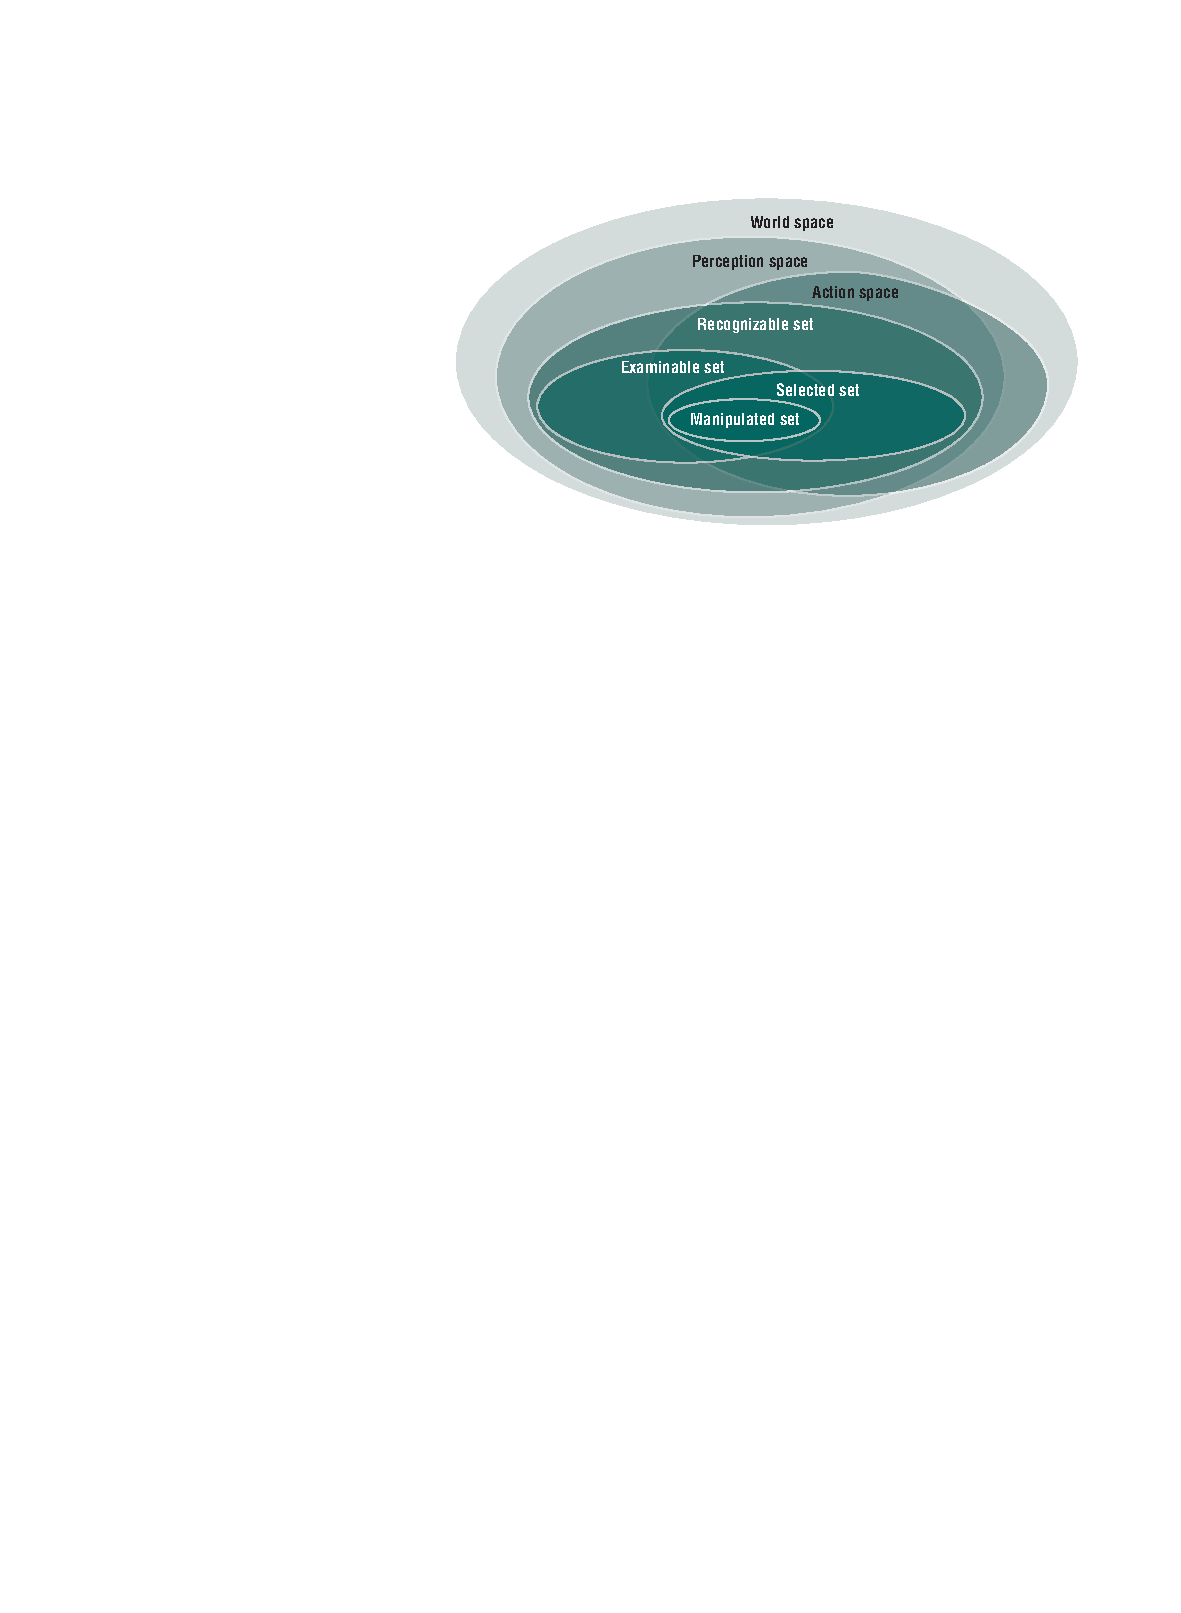
\includegraphics[width=0.7\linewidth]{gfx/Chapter3/ssm_sets}
	\caption{A situative space model (SSM). The spaces represent presence and approximate spatial relationship among physical and virtual objects with respect to what a specific human agent can perceive (perception space) and manipulate (action space) at a given moment in time. Whether objects are perceivable and manipulable depends on their relations to the human agent in all available interaction modalities (for example, vision, touch, and audio).\cite{pederson2011situative}}
	\label{fig:req_ssm_sets}
\end{figure}

As described in the definitions above, in order to correctly classify objects, they need to be augmented with the following parameters: \emph{PERCEPTION\_DISTANCE}, \emph{RECOGNITION\_DISTANCE}, \emph{EXAMINATION\_DISTANCE} and \emph{ACTION\_DISTANCE}. Normally, they should be given meaningful default values, therefore configuring them should not be a mandatory step. Even so, some objects might need adjusted values, so the possibility should be given to the system designer.
% section requirements (end)
%************************************************
\section{Challenges of building onto related systems} % (fold)
\label{sec:reusing_related_systems}
%************************************************
While researching the systems presented in the related work chapter \ref{ch:related_work}, we have analysed the possibilities of reusing some of them so we do not start from scratch. Unfortunately, none of them was fit for our approach. In this section we present the challenges we would face trying to design our solution in the context of some of the related systems.

%************************************************
\subsection{DiaSim}\label{subsec:design_diasim}
%************************************************
After thorough analysis, we found DiaSim's \ref{sec:diasim} simulation model as being generic enough to possibly host our needs. The simulation model seems to be flexible and open for further modifications. The system is not open source and the research team is not yet open for external collaboration. We have contacted the research group at INRIA\footnote{\url{http://www.inria.fr}} proposing a collaboration in order to extend DiaSim in the directions required by this project. The answer we got back is that development of DiaSim is momentarily suspended as most of the group is focused on another project. They will resume development of DiaSim only six month later. Even so, they are yet unable to determine whether a partial release of the sources is possible.\\

Even if building on top of DiaSim would have been possible, some outstanding issues should be tackled. The simulated environment does not monitor the agent's field of vision. To accommodate this need, the renderer module should be entirely replaced. Besides, there is no support for direct interaction with physical objects and mediators. The only type of interaction is proximity based: i.e. a sensor attached to a door would command the door to open if the agent is within range. Moreover, DiaSim is lacking an open API to enable third party service to make use of the simulated system's context data.\\

%************************************************
\subsection{SIMACT}\label{subsec:design_simact}
%************************************************
SIMACT \ref{sec:simact} is a smart home infrastructure simulator built to reproduce everyday life scenarios on a step-by-step basis. To make it easier to comprehend the simulated system, SIMACT animates the simulation using the jMonkey Engine (JME) framework. SIMACT is not a tool to create simulations for simulation user, rather it a simulation framework for system designer design and run simulations of homes, with the possibility of observing the system's evolution over time in an animated 3D environment.\\

Although SIMACT does not offer the necessary means to support the implementation of our requirements, the JME game engine used to animate the simulations has caught our attention. JME has all the capabilities of a modern game engine which, as discussed in this chapter, we consider well fit to accommodate our requirements. In Chapter \ref{ch:implementation} we will argue for JMonkey as a possible candidate to be used in our work.\\

%************************************************
\subsection{TATUS}\label{subsec:design_tatus}
%************************************************
TATUS \ref{sec:tatus} is a 3D simulator implemented on top of Half-Life's Game Engine. It has exploited the concept \emph{Triggers} from the SDK to simulate sensors and actuators. They are used to generate associated events based on a player's movements and location. Therefore, TATUS already has proximity detection, but only based on sensors.\\

It would be possible to partially base our design on TATUS' triggers. By attaching such a trigger to each object we would like to classify based on the agent's proximity, we would probably have out of the box distance computation. But, TATUS does not simulate interaction with devices neither does it simulate interaction with everyday physical objects. Moreover, as discussed in section \ref{sec:eval_comparison} the game engine TATUS is built upon is hard to master and get started with.\\

To conclude, TATUS is not open-source, making it unusable for research outside the institution it was developed in.\\

%************************************************
\subsection{UbiWise}\label{subsec:design_ubiwise}
%************************************************
UbiWise \ref{sec:ubiwise} was designed to simulate the interaction of the agent with the device prototypes within the target environment, not with the actual environment. Moreover, the framework empowers the user to interact with the software running on them. Therefore UbiWise handles the representation of mediators and interaction with virtual objects. This could be a good starting point. But UbiWise is solely oriented towards simulating prototyped devices. The virtual agent can interact with the prototyped devices and with the software running on them, some of the device may even be hand-held. It has no direct interaction with physical objects, the framework does no track the agent's position towards objects within the environment and does not determine the objects within the agent's field of vision. The underlying game engine might provide the necessary means to accommodate these requirements, but the effort depends greatly on individual experience in C programming.\\

To conclude, UbiWise was implemented with a radically different goal in mind and it poses an unnecessary technical challenge to try and accommodate EgoSim's requirements into its design.\\

%************************************************
\subsection{Conclusion}\label{subsec:reusing_conclusion}
%************************************************
In this section we have presented the challenges we would have faced trying to design our solution in the context of some of the related systems. None of the system were fit for our approach, but we had much to learn from them, nonetheless. Most systems which allow direct interaction between the agent and the simulated environment were build to some degree using game engines. We are considering to include game engines into our design as argued for in Section \ref{sec:simulation_runtime}.

% section sec:reusing_related_systems (end)
%************************************************
\section{Architecture} % (fold)
\label{sec:architecture}
%************************************************
In this section we will describe the high level components we have developed to accommodate the requirements described in Section \ref{sec:requirements}. To empower the system designer to set up a simulation we need a \emph{Simulation Designer}. Using the simulation designer, the system designer is able to create a \emph{Configured Environment Model}, where all the objects of interest for the simulation have been identified and configured. The \emph{Simulation Runtime} loads a configured environment model and enables the simulation user to control an \emph{Avatar} in order to interact with the environment. As the agent interacts with the environment, the \emph{Context Manager} monitors the agent's position and visual spectrum, delegating the classification of objects around the user to the \emph{SSM Classifier}. The \emph{SSM Sets} can be visualized in the \emph{Context Client} and can be accessed through the \emph{API}.\\

For a better overview, the proposed architecture is illustrated in Figure \ref{fig:initial_architecture}.

\begin{figure}[H]
	\centering
	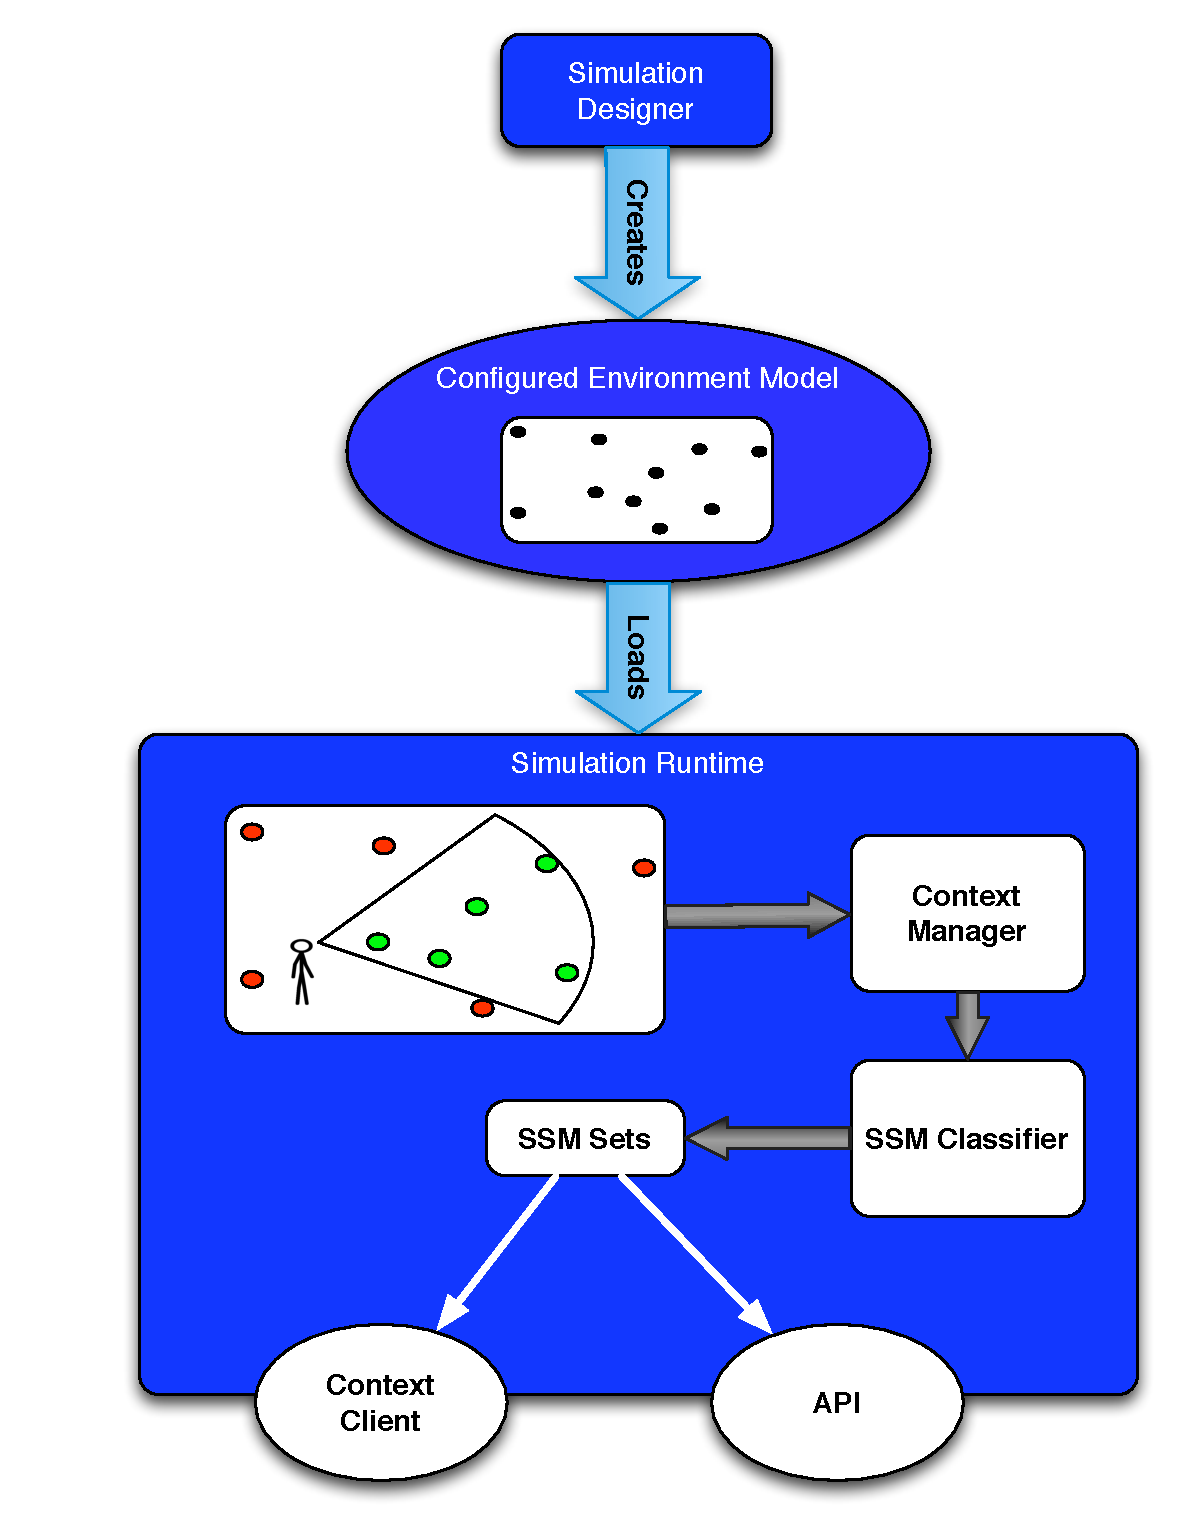
\includegraphics[width=0.8\linewidth]{gfx/Chapter3/initial_architecture}
	\caption{EgoSim Architecture Diagram}
	\label{fig:initial_architecture}
\end{figure}
% Describe the big picture in words and using a picture as well! Describe the main components imposed by this architecture: 3D modelling (to represent the space), rendering and movement control to build the simulated environment, categorization algorithms AND programming API (including the ContextClient).\\

% In the remaining of this chapter good deep into details about why I've chose certain technologies for each component; put each discussion in its own section! To better argue, present several technologies that could fit the same requirements and argue objectively about the the reasons I've made certain choices. I should refer back to arguments in the related work!

% section architecture (end)
%************************************************
\section{Simulation Designer} % (fold)
\label{sec:simulation_designer}
%************************************************
\subsection{Environment Modelling}\label{subsec:environment_modelling}
\subsection{Object Properties}\label{subsec:object_properties}
% section simulation_designer (end)
%************************************************
\section{Simulation Runtime} % (fold)
\label{sec:simulation_runtime}
%************************************************
\subsection{The Agent}\label{subsec:agent}
\subsection{The Environment}\label{subsec:environment}
\subsection{The Monitoring Service}\label{subsec:monitoring_service}
\subsection{The API}\label{subsec:api}
\subsection{The ContextClient}\label{subsec:context_client}
% section simulation_runtime (end)
%************************************************
\section{The Agent} % (fold)
\label{sec:the_agent}
%************************************************
The agent is the active entity the simulation user can control, using various input mechanisms, in order to interact with the environment. In 3D games and simulations, there are two main graphical perspectives employed to interact with the environment -- the first-person and third-person perspectives. These perspectives are the result of positioning the camera in a certain manner, providing a different perception of the environment. To control the agent's position and orientation, the camera's position and direction are coupled to a set of input controls. As the camera is moved and rotated, it creates the impression of interaction with the 3D environment. For a more realistic interaction, various animations are carried out.

\subsection{First-Person}\label{subsec:first_person}
The first-person view is a graphical perspective rendered from the viewpoint of the agent. Figure \ref{fig:fps} illustrates the first-person view from a running simulation built with Tatus \cite{o2005testbed}.

\begin{figure}[H]
	\centering
	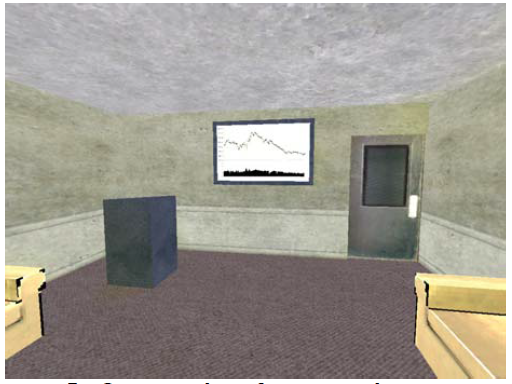
\includegraphics[width=\linewidth]{gfx/Chapter3/fps}
	\caption{A first-person perspective}
	\label{fig:fps}
\end{figure}

Using this perspective, the simulation displays what the simulation user would see with the agent's own eyes thus, objects have to be scaled accurately to appropriate sizes. It doesn't deserve a paragraph by itself.\\

In this perspective, the simulation users typically cannot see the agent's body, although it might be helpful for the user to see the agent's hands. On the plus side, there is no need for sophisticated animations for the agent, which reduces development time. Also, it helps for easier, more realistic aiming (pointing at objects to interact with) since there is no representation of the avatar to block the simulation user's view. Not seeing the agent's body reduces development efforts, but might represents a drawback as well.\\

\subsection{Third-Person}\label{subsec:third_person}
The third-person view is a graphical perspective rendered from a fixed distance behind and slightly above the virtual agent. The third-person perspective can provide an animated, strong characterized agent, directing the simulation agent's attention as she/he were watching a film.\\

On the plus side, the third-person perspective allows the simulation user to see the area surrounding the agent more clearly. This viewpoint facilitates more interaction between the virtual agent and their surrounding environment.\\

As a drawback, the third-person perspective can interfere with accurately pointing at objects, as the agent's body might block the simulation user's view. Moreover, implementing this perspective takes a lot more effort as the there is a need for an animated agent body and for custom code to make the camera follow the agent within the simulation.\\

\subsection{Discussion}\label{subsec:agent_discussion}
Based on the preceding review of existing perspectives, we have decided to include in our design a first-person perspective for the agent. An argument for choosing this perspective is that a first-person view provides the simulation user with greater immersion into the simulated environment.\\

Avatar based games and simulations usually provide both views, with an easy way to switch perspectives during runtime. For this project, a third-person perspective could be useful for future work if we are to represent wearable devices. Also, it enables the simulation user to observe the various body gestures the agent is doing.\\

To fully support requirement \ref{us:4}, we need to define a way of controlling the agent. Most games and simulations use a combination of the keyboard and the mouse to control the agent. The standard control combination is described bellow:
\begin{itemize}
	\item moving \emph{the mouse} controls the agent's direction; hence mouse movements translate into rotating the agent's viewpoint within the environment. This control is used to look around and to point at objects the simulation user desires to interact with
	\item clicking \emph{the left mouse button} triggers an interaction. The interaction is contextual; for example, clicking on a switch will turn on or off the switch. If the user clicks on a pen, the agent would pick the pen up, while if the user clicks on a surface while the agent is carrying a pen, the agent will put the pen onto the surface. Of course, the ability to carry out these actions depends on the distance between the object and the agent.
	\item moving the agent is done by activating a set of four keys on the keyboard. We have chosen the standard W, A, S, D key combination. Each key move the agent towards a certain direction, Therefore, W - forward, A - left, D - right, S - backward.
\end{itemize}

To help the simulation agent with the task of accurately aiming at objects, a cross icon will always be present in the middle of the screen. The object currently pointed at will represent the object the user intends to interact with.\\

In order to determine the object to interact with, we use the concept of \ref{ray_casting}. To achieve this, we cast a ray of infinite length from the current location of the camera along it's direction. This ray passes right through the middle of the cross and intersects all the objects along the way. We then determine the object to interact with by picking the closest object to the agent; that is the first object intersected by the ray. Moreover, the object can be interacted with only if it carries Ego metadata, otherwise the interaction is not possible. We have imposed this constraint because without the meta-data we cannot take concrete decision on what to do with the object.\\

Whether an object can be interacted with or not, is given by the current distance towards that object. Therefore, the distance has to be at most equal to the value of the ACTION\_DISTANCE property in the in the metadata.\\

Finally, the agent should not be able to pass through walls and other physical objects. Game engines provide various mechanisms for collision detection that can be used in the implementation to accommodate this aspect.\\
% section the_agent (end)
%************************************************
\section{Monitoring Service} % (fold)
\label{sec:monitoring_service}
%************************************************
The purpose of the monitoring service component is to keep track of the objects marked with Ego metadata and classify them into SSM sets, as the simulation user controls the virtual agent to interact with the surrounding environment. In order to classify the objects, the service needs the following data: the agent's location and agent's orientation, the objects within the agent's field of vision and the Ego metadata of the monitored objects.\\

Next, we will briefly address how to determine whether objects are within the agent's filed of vision or not, followed by separate discussions on how the framework categorizes the objects into various SSM sets. The sets have been defined in Section \ref{subsec:ssm_params}.\\

%************************************************
\subsection{World Space}\label{subsec:world_space}
%************************************************
Central to all computations and decisions in this framework is the World Space. It is ought to contain all the objects in the environment carrying Ego metadata. To design for easy access to the objects carrying Ego metadata, when the simulation is started up, we parse the \ref{scene_graph} and each object carrying Ego metadata is added to the World Space. Whenever we need to categorize the monitored objects, we can simply refer to the World Space.\\

The drawback of this choice is that we are duplicating a set of data already present in the scene graph. The advantage is that we don't have to parse to \ref{scene_graph} every time we are interested in the objects carrying Ego metadata; accessing them from a reduced set of data brings performance improvements. Moreover, the World Space has to always be available through the API and it never changes, so computing it once, at the simulation's start-up, comes as a natural decision.
% subsection world_space (end)

%************************************************
\subsection{Objects within field of vision}\label{subsec:visible_objects}
%************************************************
To determine the objects within the agent's field of vision, we can rely on the agent's \ref{view_frustum} and the World Space \ref{subsec:world_space}. The frustum describes six planes: top, bottom, left, right, near and far. If the object is fully contained within or partially intersects the view frustum, we can consider the object is within the agent's field of vision. This is the same algorithm game engines use to determine whether to render or not a certain object (a process called culling).\\

The solution above does leave us one problem though: occluded objects will be considered visible. An object is considered to be occluded if other objects are in front of it blocking the agent's visibility over the target object.\\

To determine if an object is occluded, we have used \ref{ray_casting}. We are casting a ray from the agent's location (the agent's position vector) to the centre of the object (the object's position vector). If the ray intersects any other object before the target object, we consider it as being occluded, therefore not in the agent's field of vision.\\

This approach should work most of the time, but there are some edge cases with false positives. For example, a small object could be positioned in front of a really large object. Even if the centre point is occluded, the agent should still be able to perceive the object as it is large enough to recognize it based on all the details it provides. To overcome these kind of edge cases, we could cast a large number of rays to various points on the object and based on a more advanced algorithm, determine if the object is being occluded. We have decided to leave the design of a more advanced computation for future work, as the current solution is good enough to cover most of the cases, while developing a more advanced and correct algorithm needs more research in the field of 3D modelling and rendering.\\
% subsection objects_within_field_of_vision (end)

%************************************************
\subsection{Categorisation into SSM spaces}\label{subsec:categorisation_ssm_spaces}
%************************************************
We have addressed the World Space \ref{subsec:world_space} separately as most of the logic of the monitoring service revolves around it. We have addressed the reset of the SSM spaces in this section.\\

To determine whether an object is part of a particular SSM space or not, we need to know the distance to that object. The distance can be computed knowing the intersection of a ray cast from the agent's location to the target object. To avoid doing the same thing twice, this computation is part of the process where we determine if the object is within the agent's field of vision, as discussed in Section \ref{subsec:visible_objects}. There, we set a the distance in the Ego metadata as the \emph{LAST\_MEASURED\_DISTANCE} property.\\

Computing the distance as described above, brings up the same discussion we had in the previous Section \ref{subsec:visible_objects} about the occlusion of objects. It is based on the same algorithm so we compute the distance to the centre of the object. This can be improve in future work, along with the algorithm for detection of object occlusion.\\

Having all the necessary parameters, Perception Space, Recognition Set, Examinable Set and Action Space are computed as described in Section \ref{subsec:ssm_params}. We have used a less generic definition of these spaces than originally defined in \cite{pederson2011situative}, but future work could broaden them up to provide a classification closer to the ones defined in the theoretical framework. For example, an object in the Perception Space can be perceived as different entities depending on the distance to the agent. Given a hammer, from the furthest perception distance (X1) the agent would perceive it as an object; from a closer distance (X2), the agent would perceive it as an object certain kind of shape while from a more closer distance (X3),  the agent would perceive it as hammer. So, an object should be perceived in different ways based on the agent's proximity. Such improvements to the classification into the aforementioned sets, are target of the future work.\\

The Selected Set contains objects currently being physically manipulated. This happens when the agent picks an object up. In order for the agent to pick up a certain object, she/he must be targeting it (aim at it with the on screen arrow) and click the Left Mouse Button (pick up action); also, the object must be in the Action Space.\\

In the current design we only support pick-up/put-down as interaction with objects in the surrounding environment. Therefore, the only manipulation the agent is empowered to do is to pick objects up and move them around. That is why in the current work, the Manipulated Set completely overlaps the Selected Set.\\

Categorisation is triggered by the agent movements. Hence, every time the agent is moved or is looking around, using the controls described in Section \ref{sec:the_agent}, a new categorisation is triggered and the SSM sets are refreshed.\\
% subsection perception_space (end)

%************************************************
\subsection{Monitoring Service Summary}\label{subsec:monitoring_service_summary}
%************************************************
To summarize, in this section we described the design for object classification into SSM sets. It comes as a solution to requirement \ref{us:6}, classifying objects around the agent as the agent's field of vision changes and as the agent interacts with the environment.
% subsection subsec:monitoring_service_summary (end)

% section monitoring_service (end)
%************************************************
\section{The API} % (fold)
\label{sec:api}
%************************************************

1. RESTful\\
2. vs others\\

% section api (end)
%************************************************
\section{The Context Client} % (fold)
\label{sec:context_client}
%************************************************
To make it easy for the simulation user to follow the evolution of the SSM Sets as the simulation unfolds and the agent interacts with the environment, as discussed in requirement \ref{us:8}, we have designed the Context Client as a service working on top of the API \ref{sec:api}. It is really just a nicely formatted visualization for easy understanding of what's going on under the hood. To provide a close to real-time visualisation, the context client will be accessing the API every second to display an updated visualization of the SSM Sets. In future work, the context client is meant to be improved alongside the API.\\
% section context_client (end)
%************************************************
\section{The Design} % (fold)
\label{sec:the_design}
%************************************************
To summarize, we present an overview of our design. We will represent the target environment as a 3D virtual model \ref{sec:simulation_designer}. We will build a simulation runtime based on a game engine \ref{sec:simulation_runtime}. To empower the simulation user to interact with the environment, we will build an agent based on a first-person perspective. The agent will be controlled using standard game controls as described in Section \ref{sec:the_agent}. As the agent is interacting with the environment the monitoring service \ref{sec:monitoring_service} will classify objects around the agent according to the Situative Space Model (SSM). The content of the SSM sets will be available for third party services through a RESTful API \ref{sec:api} and for the simulation user, in a visual representation, through the context client \ref{sec:context_client}. Figure \ref{fig:final_architecture} show a visual overview of this design. It is a more concrete design than the one presented in the begging of this chapter \ref{fig:initial_architecture}. We have modified the initial design to fit the architecture of a game engine illustrated in Figure \ref{fig:game_engine_architecture}.
\begin{figure}[H]
	\centering
	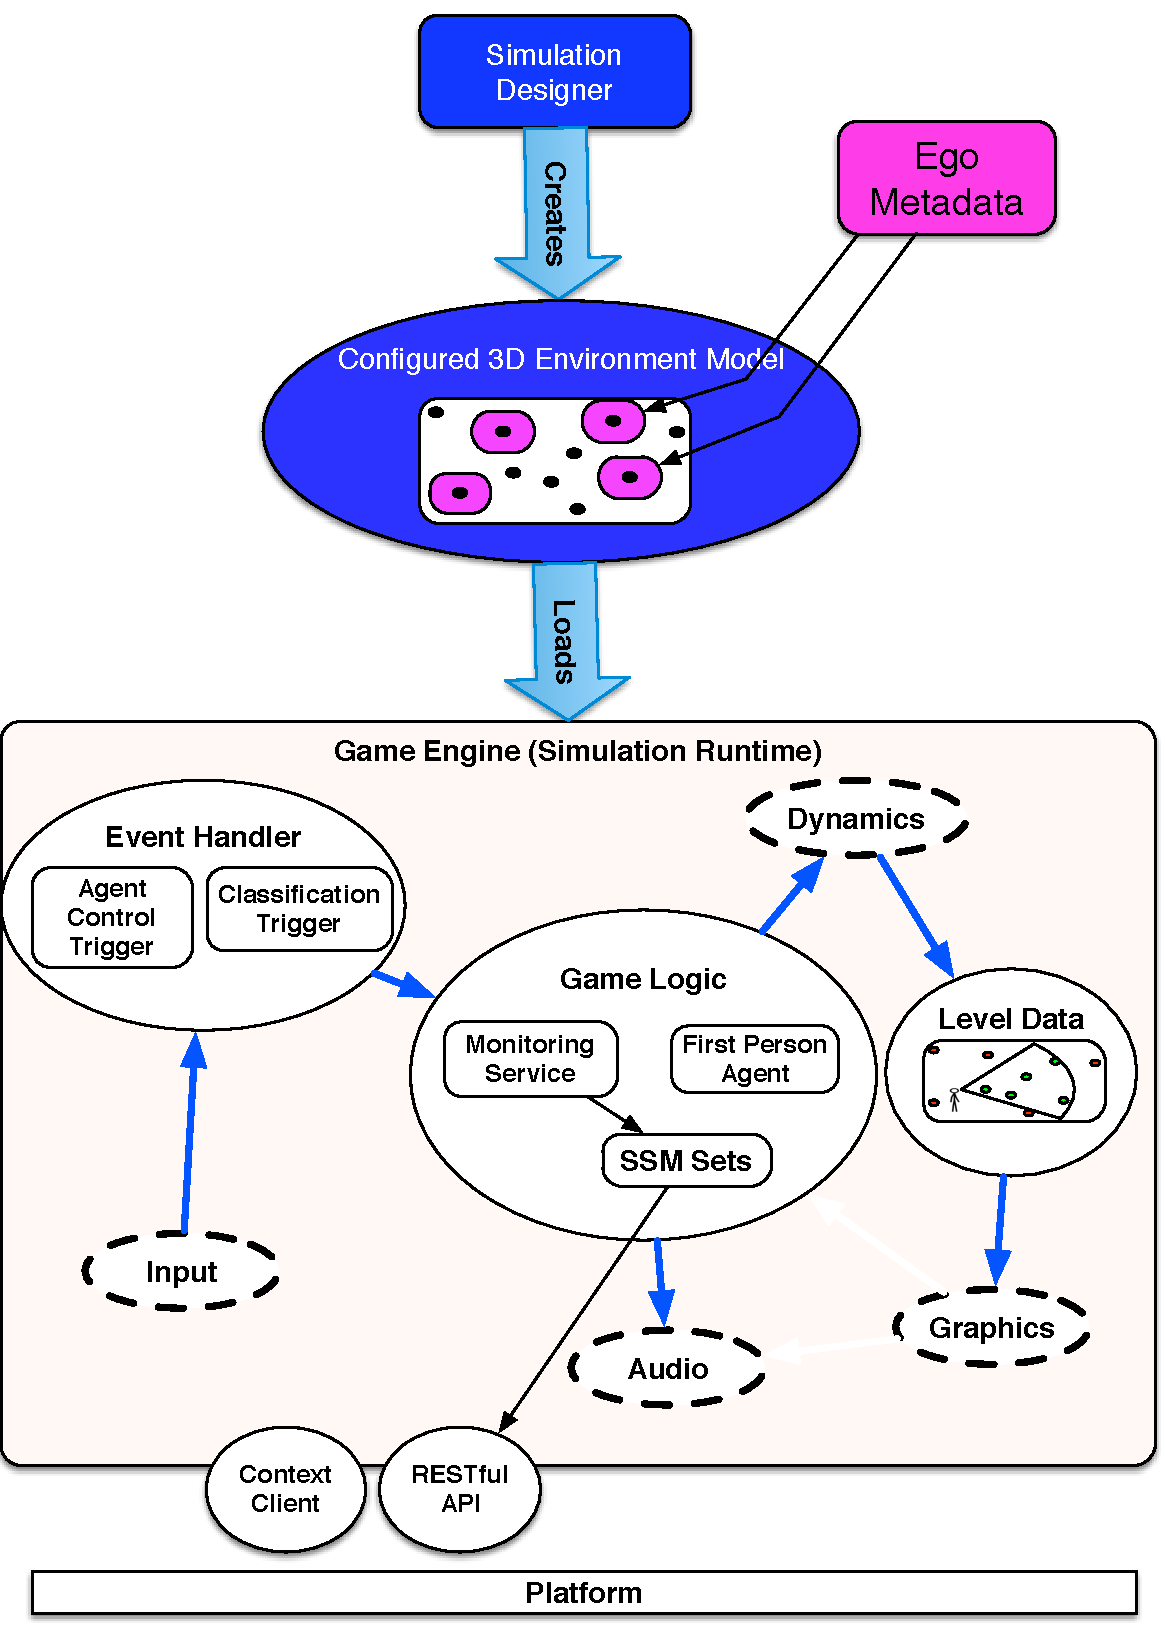
\includegraphics[width=\linewidth]{gfx/Chapter3/final_architecture}
	\caption{EgoSim: A visual overview of our final architecture}
	\label{fig:final_architecture}
\end{figure}
% section the_design (end)

% \begin{enumerate}
% 	\item Follow a modular design to implement the core of the framework as a set of decoupled components:
% 		\begin{itemize}
% 			\item The \emph{Data Model}. This represents the contextual entities and the relationship between them that the simulator will monitor, briefly detailed in Section \ref{sec:data_model}.
% 			\item The \emph{World Model}. Represents the current status of the simulated environment (e.g. position of the agent, status of a certain switch etc.). The structure of the entities in this model have been defined in the Data Model.
% 			\item A universal communication protocol to access the core. It needs to be universal so that other components, can easily be developed and integrated.
% 			\item Query and modify API of information in the World Model. To make the integration between the core of the framework and the other modules, these APIs will need to provide a complete set of methods.
% 		\end{itemize}
% 	\item Evaluate the framework:
% 		\begin{itemize}
% 			\item Implement a module to modify the state of the simulated environment (DummySim). This comprises of manipulating the agent's parameters and performing actions like picking up an item, touching a screen etc. The purpose of this module is to evaluate the modify API of the core. It also servers as a tool to modify the environment which is a required input for the SSM model to be evaluated.
% 			\item Implement the \emph{SSM Model}. Using the current World Model's query API, retrieve the current set of contextual data and apply the rules defined in the SSM. This component will actively monitor the current status of the simulator, having as a result an up to date collection of SSM entity sets: world space, perception space, recognizable set, examinable set, action space, selected set and manipulated set. This evaluation will be considered successful if the results are similar to the results obtained in the initial evaluation of the SSM described in \cite{pederson2011situative}.
% 		\end{itemize}
% \end{enumerate}


% In order to allow the user of the simulator to easily interact with the simulated environment, the visualization is really important. Projects that simulate real world scenarios, employ game alike solution providing complex graphics and interaction between the user of the simulator and the simulated world.\\

% This work represents initial research for this egocentric simulator. Therefore, my main focus is on the framework's core. But, I will invest time in researching existing solutions, either 2D or 3D; if I will document the suitable frameworks with high potential. This is nice-to-have. I don't want to set it as a goal of this project, rather talk about it as future work.

% \subsection{Data Model}\label{sec:data_model}
% The data model is aimed at defining the supported entities and the relationships between them. In this work the aim is to support physical objects, virtual objects and mediators.\\

% The agent represents a virtual character that can freely moved around in the environment. Beside the position the of the agent, the user can also control more complex parameters of the agent like orientation (affects field of vision), sitting down / standing, hands orientation etc. The agent will be also be able to carry out a certain set of actions like picking objects up, putting objects down etc.\\

% Physical objects will be described as entities with a certain set of properties (location, weight etc.). Entity composition will be supported to some extend: place objects on top of each other (i.e. a stapler on a table), a mobile phone in the backpack worn by the agent.\\

% This section created a brief overview of the supported entity types and relationships. They will be described in details in Chapter \ref{ch:design}.